\documentclass{article}
\usepackage{amsmath}
\usepackage{amsfonts}
\usepackage{hyperref}
\usepackage[english,russian]{babel}
\usepackage{graphicx}

\DeclareMathOperator{\grad}{grad}
\newcommand{\divg}{\mathrm{div}\,}

\begin{document}
	
\section{Постановка задачи}
Решается двумерная задача Дирихле для двумерного стационарного оператора диффузии

$$
\begin{cases}
    \divg(-\mathbb{D} \grad u) = f, x \in \Omega, \\
    u|_{\partial \Omega} = g.
\end{cases}
$$
$
    \Omega = [0,1]^2, D = diag(d_x, d_y).
$

Задача решается методом конечных элементов на треугольной сетке. Интерполяция происходит классическими линейными базисными элементами. Интегралы по треугольникам берутся численно с помощью квадратурной формулы.

Работа с сеткой, а также решение получившейся системы происходит с помощью библиотеки \href{https://github.com/INMOST-DEV/INMOST}{INMOST}.


\section{Численный эксперимент}

Эксперимент проводился для задач, в которых известно аналитическое решение, а именно
\begin{enumerate}
	\item $f = \sin(\pi x) \sin(\pi y), d_x = d_y = 1$. $u = \frac{\sin(\pi x) \sin(\pi y)}{2 \pi^2}$.
	\item $f = \sin(10 x) \sin(10 y), d_x = d_y = 1$. $u = \frac{\sin(10 x) \sin(10 y)}{200}$.
	\item $f = \sin(4 x) \sin(4 y), d_x = 5, d_y = 1$. $u = \frac{\sin(4 x) \sin(4 y)}{16(d_x + d_y)}$.
\end{enumerate}

Заметим, что во втором случае краевое значение является неоднородным. Также в третьем случае тензор диффузии является неоднородым.

Для всех трех экспрементов построены графики С-нормы и L2-нормы отклонения при сгущении сетки.

\begin{figure}[h!]
	\centering
	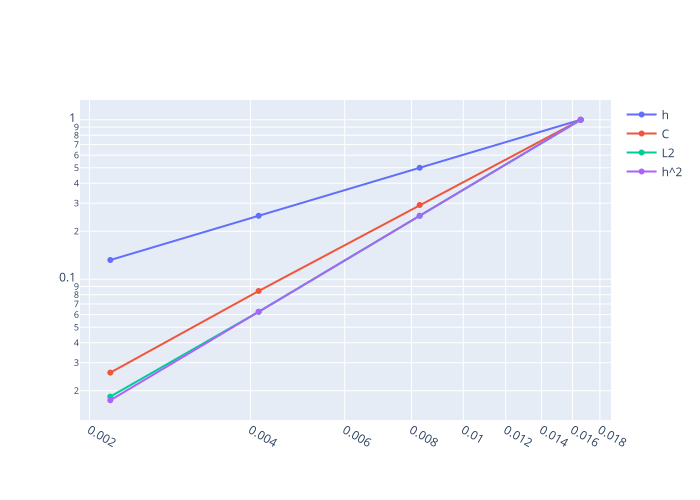
\includegraphics[width=.9\textwidth]{img/res1.png}
	\caption{$f = \sin(\pi x) \sin(\pi y), d_x = d_y = 1$}
\end{figure}

\begin{figure}[h!]
	\centering
	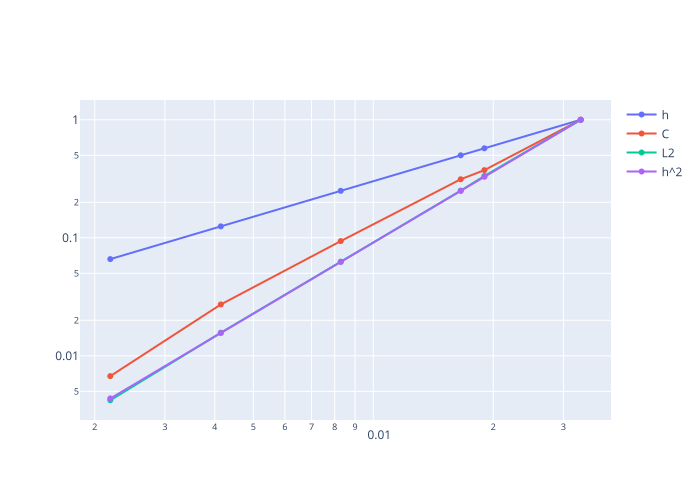
\includegraphics[width=.9\textwidth]{img/res2.png}
	\caption{$f = \sin(10 x) \sin(10 y) , d_x = d_y = 1$}
\end{figure}

\begin{figure}[h!]
	\centering
	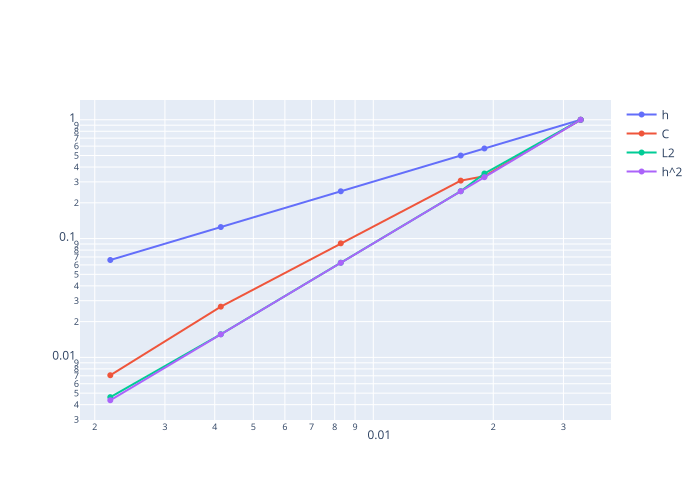
\includegraphics[width=.9\textwidth]{img/res3.png}
	\caption{ $f = \sin(4 \pi x) \sin(\pi y), d_x = 5, d_y = 1$}
\end{figure}


\begin{figure}[!htb]
	\minipage{0.33\textwidth}
	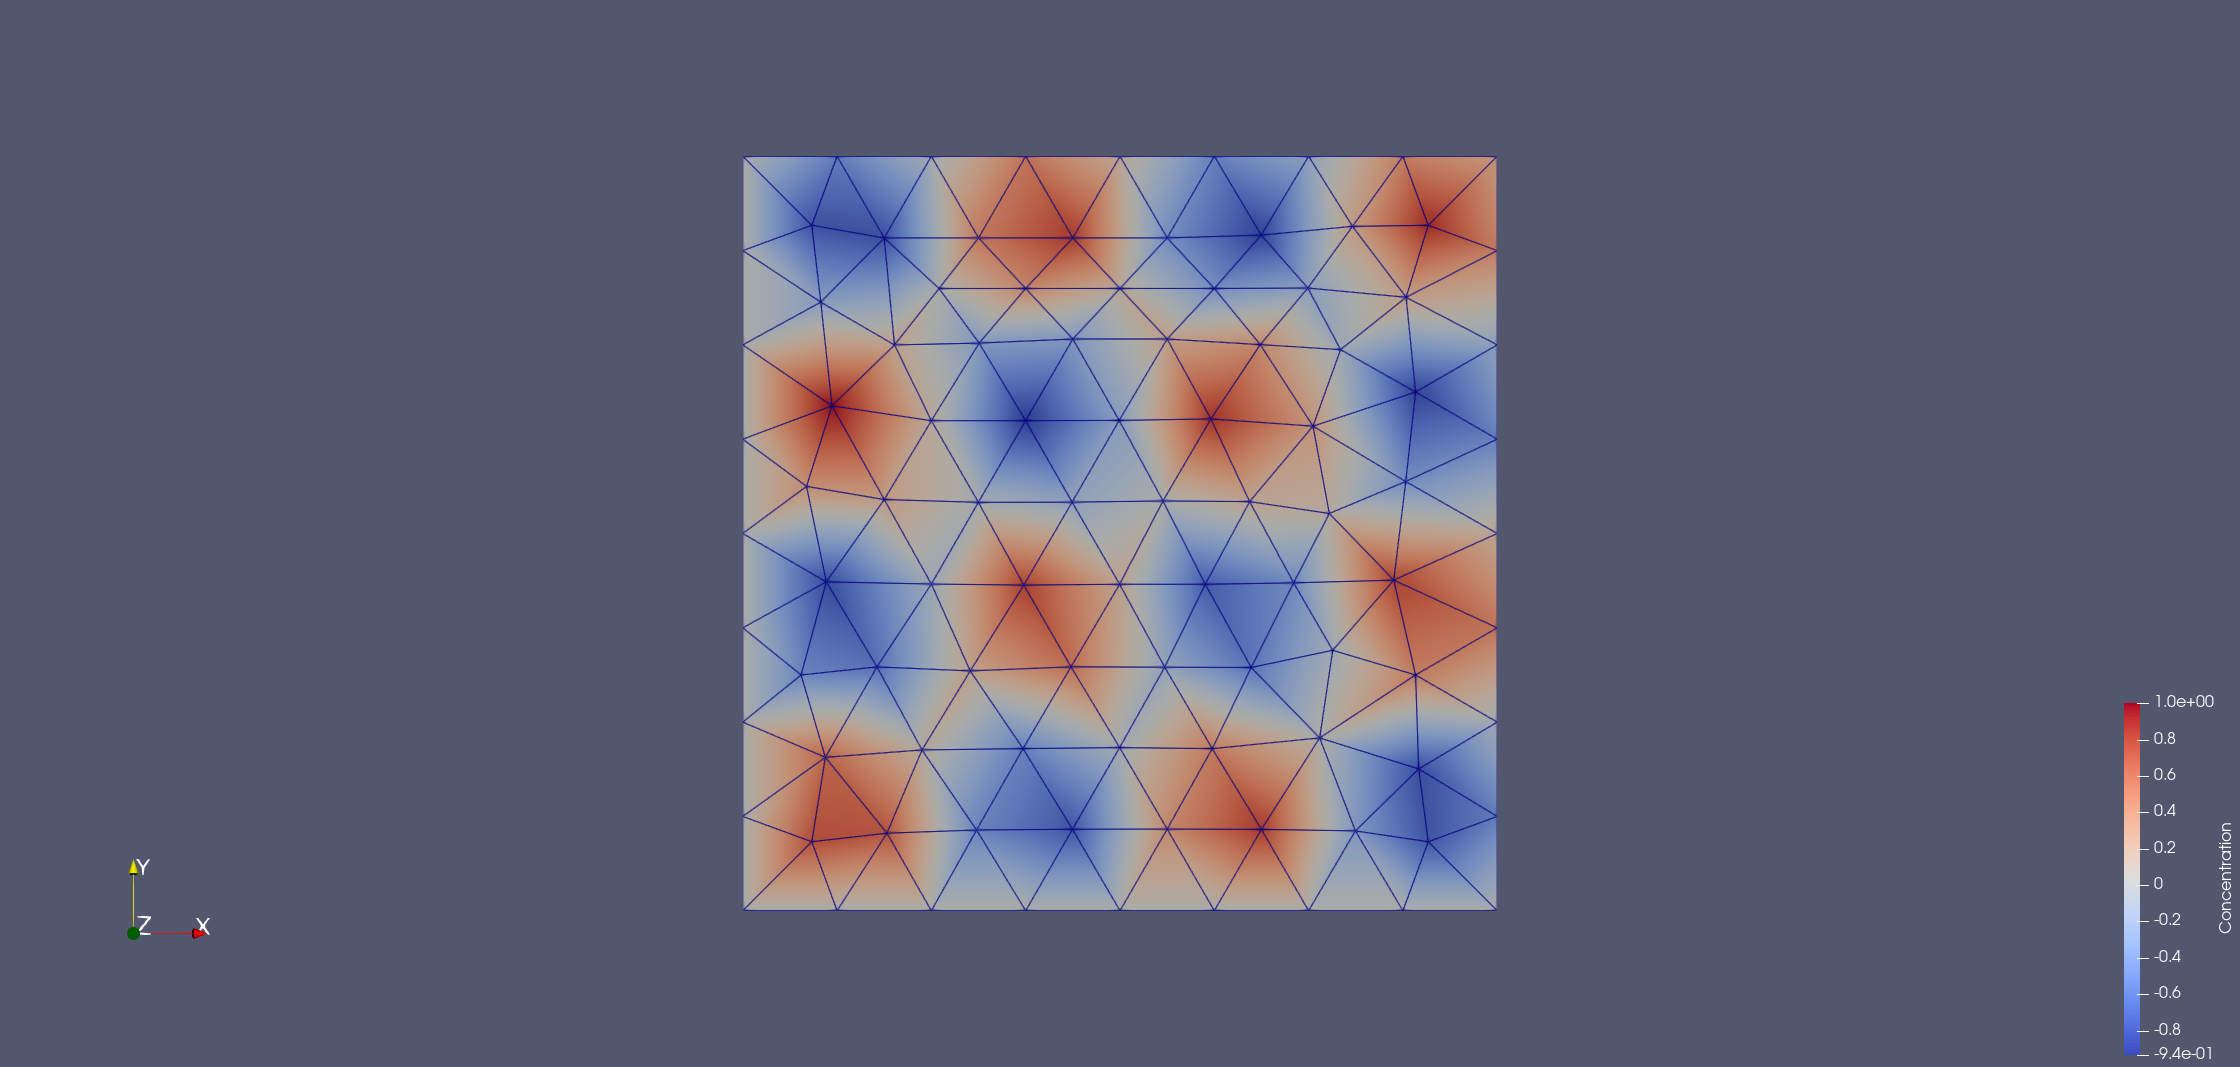
\includegraphics[width=\textwidth]{img/32.png}
	\caption{$u, d = 0.15$}
	\endminipage\hfill
	\minipage{0.33\textwidth}
	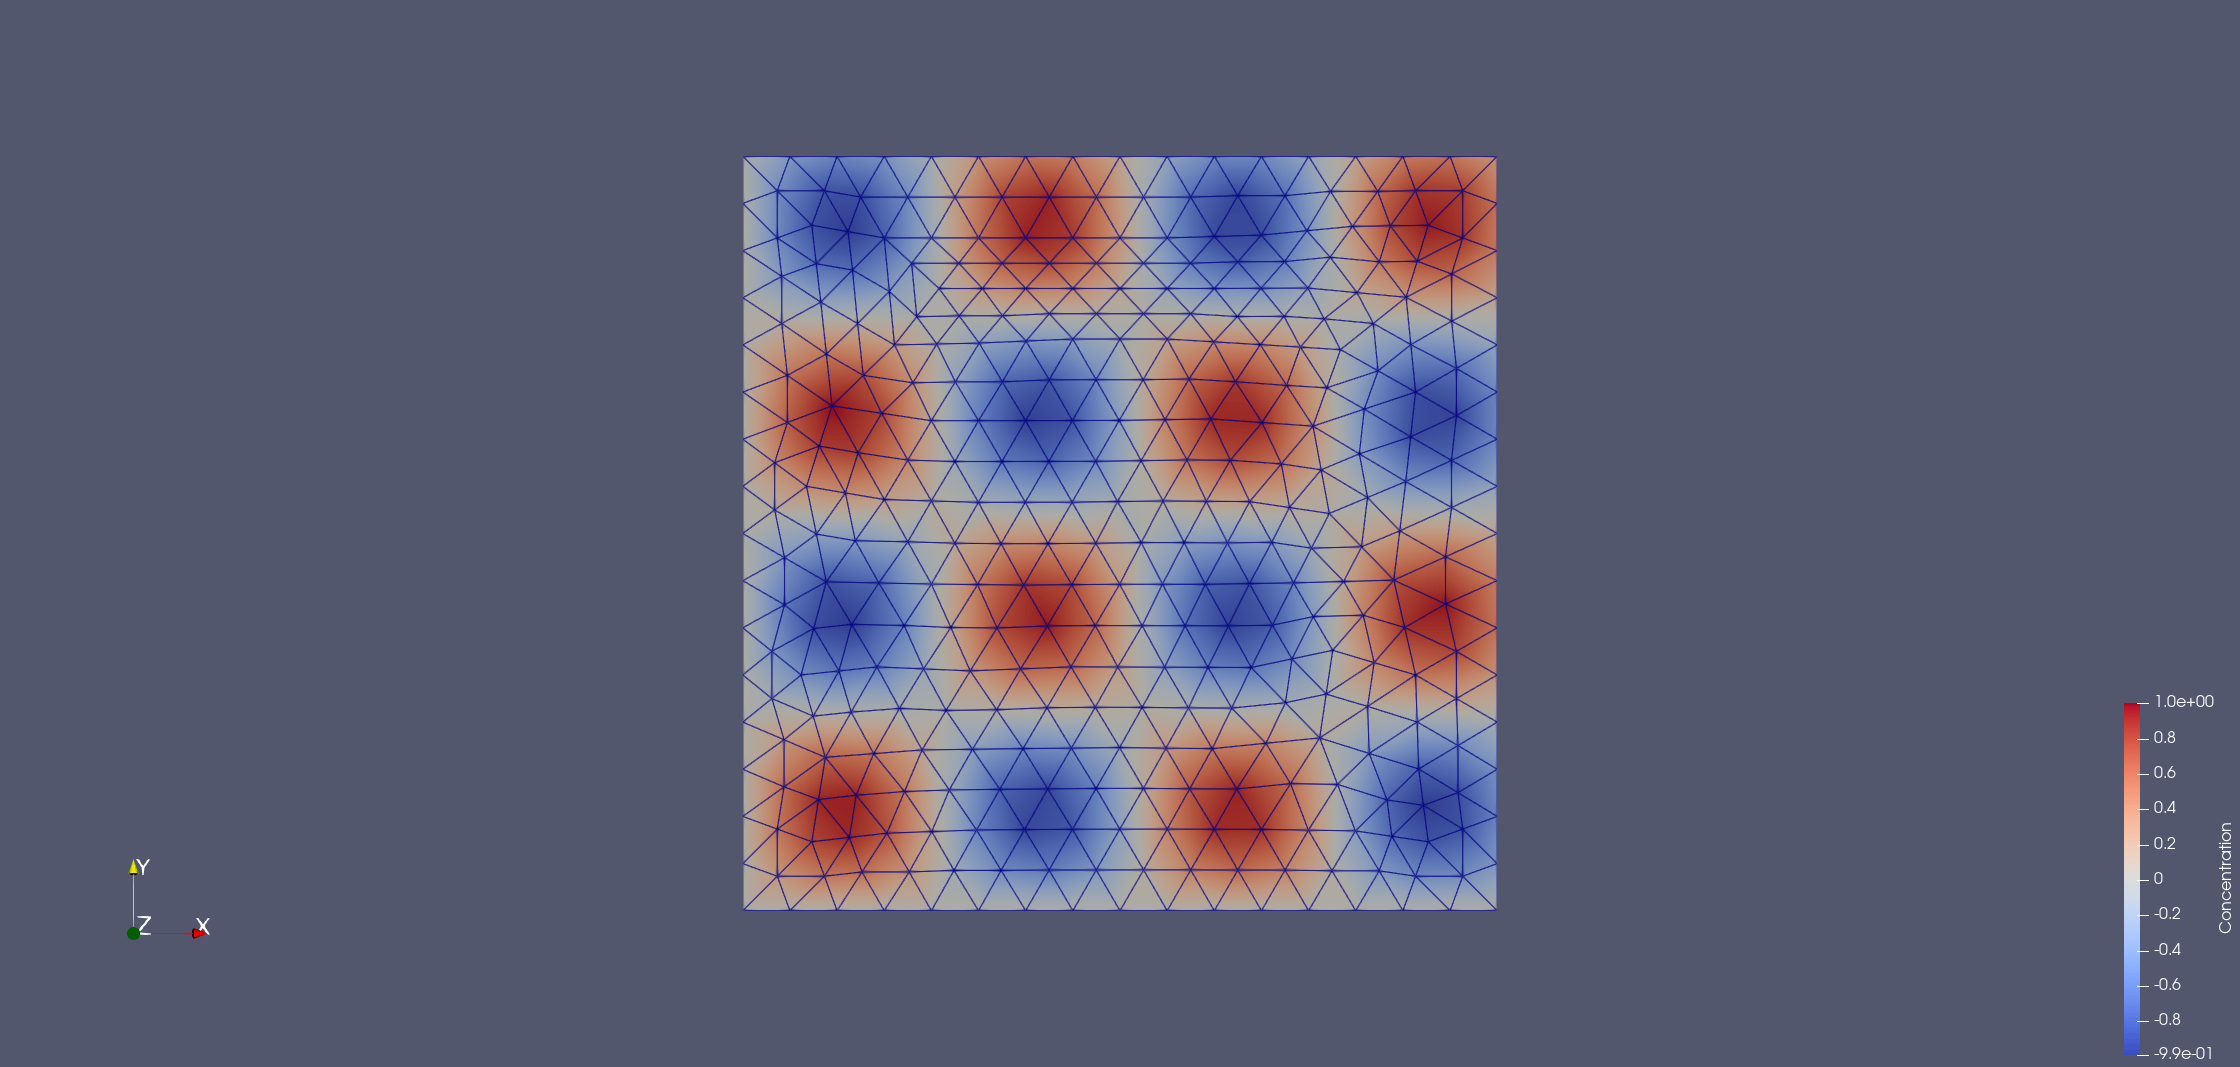
\includegraphics[width=\textwidth]{img/64.png}
	\caption{$u, d = 0.076$}
	\endminipage\hfill
	\minipage{0.33\textwidth}%
	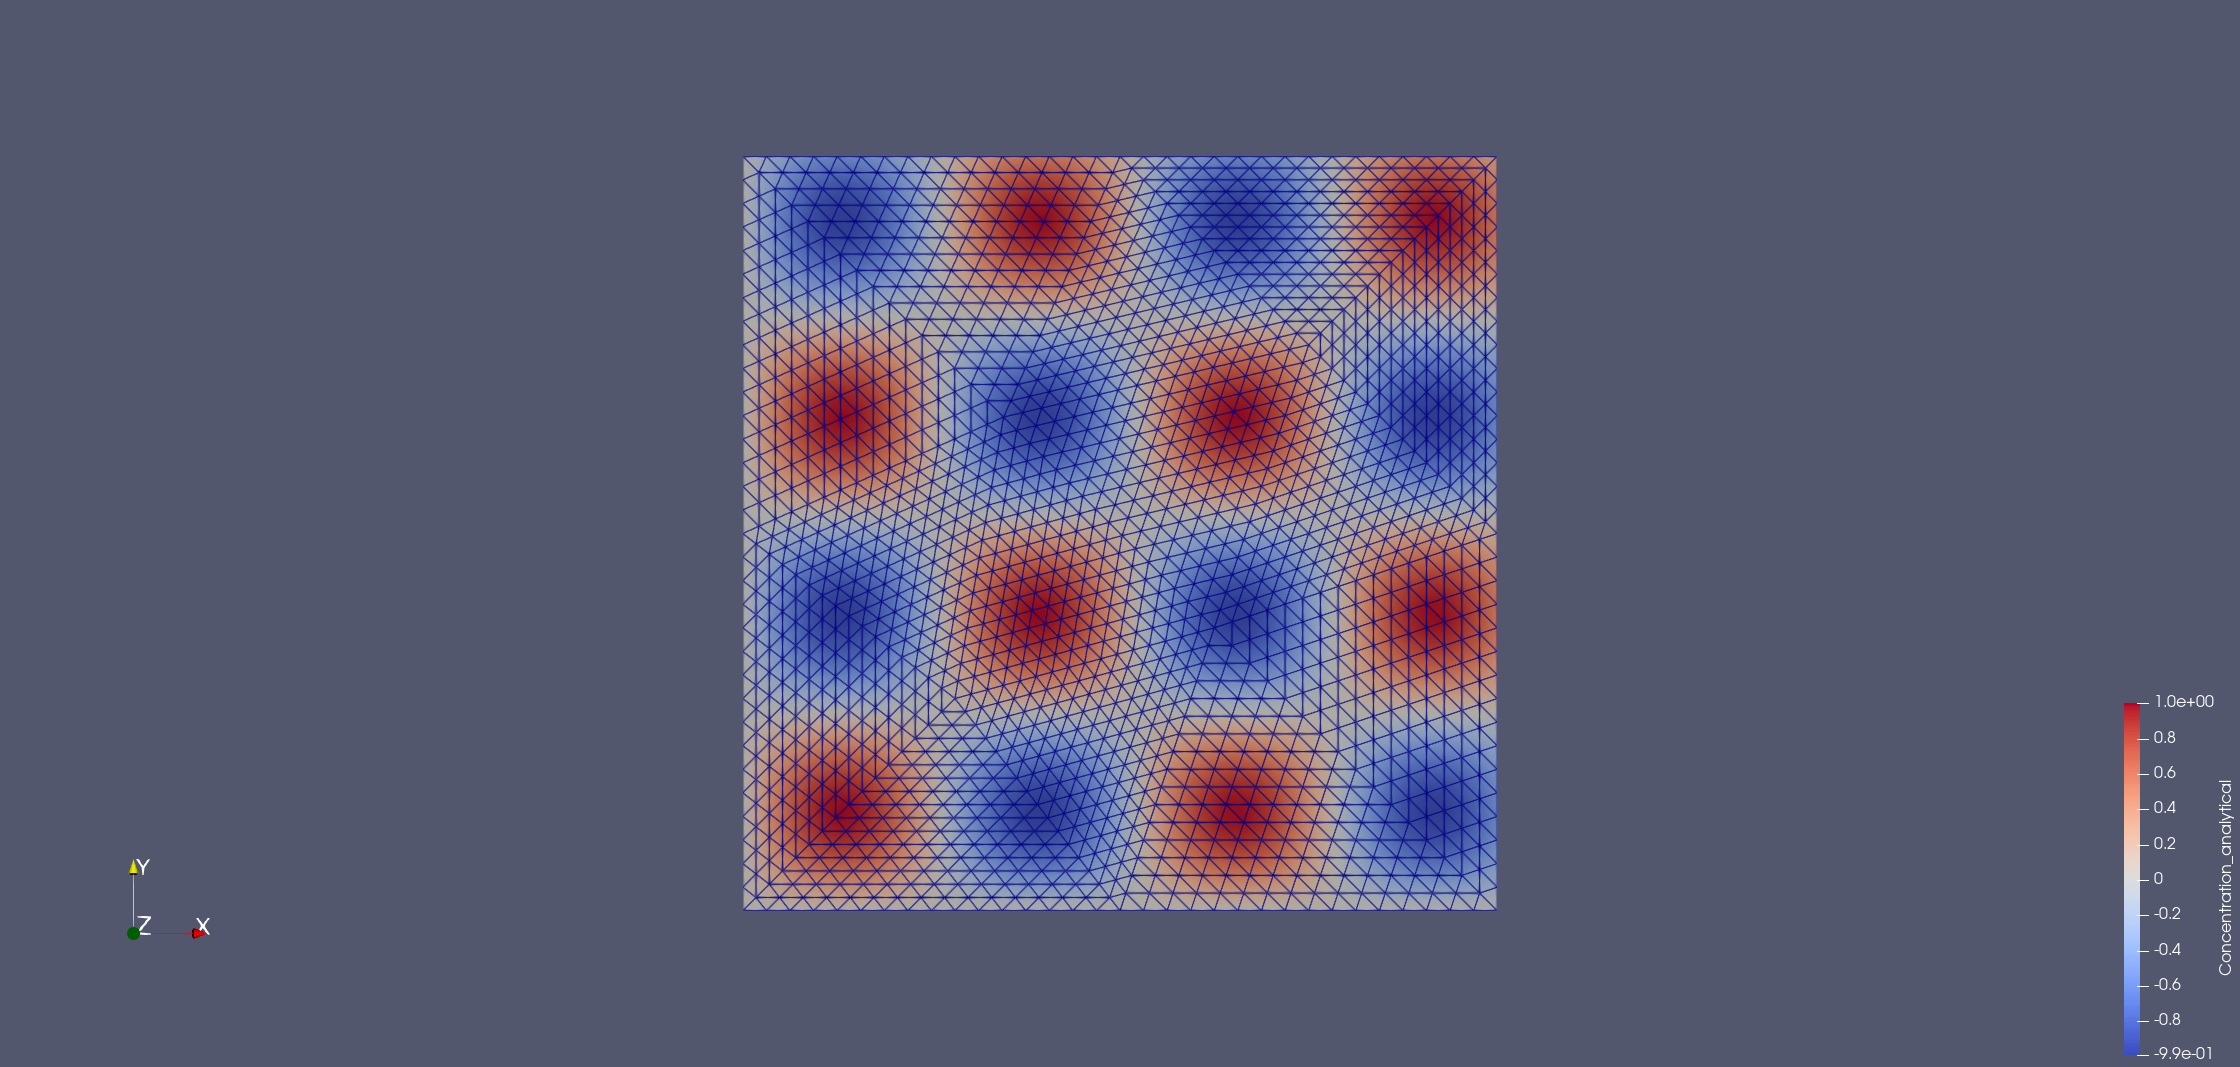
\includegraphics[width=\textwidth]{img/128.png}
	\caption{$u, d = 0.003$}
	\endminipage
\end{figure}

\end{document}